% !TEX root = ../main.tex
\Chapter{Methods}
\label{chap:methods}

\section{Overview}
This work implements a modular pipeline for systematic augmentation and assessment of predicted protein structures using experimentally resolved homologous complexes and associated ligands. The architecture consists of (i) structured acquisition of target and donor structural data, (ii) detection and characterization of binding environments, (iii) sequence/structure alignment and geometric mapping, (iv) ligand and pocket feature transplantation with conflict resolution, (v) multi-criteria filtering and scoring, and (vi) standardized evaluation and visualization of resulting models and annotations. This layered decomposition promotes separation of concerns, controlled extensibility, and reproducible execution.

Inputs consist of one or more target protein identifiers (e.g., UniProt accessions) whose corresponding predicted three-dimensional models are retrieved (or validated if cached) and normalized. Donor candidates are gathered from curated structural repositories and homolog databases according to configurable similarity, coverage, and quality constraints. Auxiliary metadata (ligands, binding site residues, cavity descriptors, and experimental provenance) are harvested through dedicated tool adapters. Each external data source is encapsulated behind a dedicated integration component to isolate protocol specifics from core orchestration logic.

Evaluation utilities quantify improvement and reliability through metrics such as structural alignment quality, pocket conservation, ligand retention integrity, and scoring distribution profiles. Visualization components generate comparative plots and summary artifacts to support interpretability and methodological diagnosis. Configuration management and structured logging ensure parameter traceability, deterministic re-runs, and auditability of intermediate decisions. The overall design facilitates insertion of new data sources, scoring strategies, or analytical endpoints with minimal impact on existing workflow stages.

\begin{figure}[H]
    \centering
    % Placeholder: replace with actual pipeline diagram (e.g., TikZ or imported PDF)
    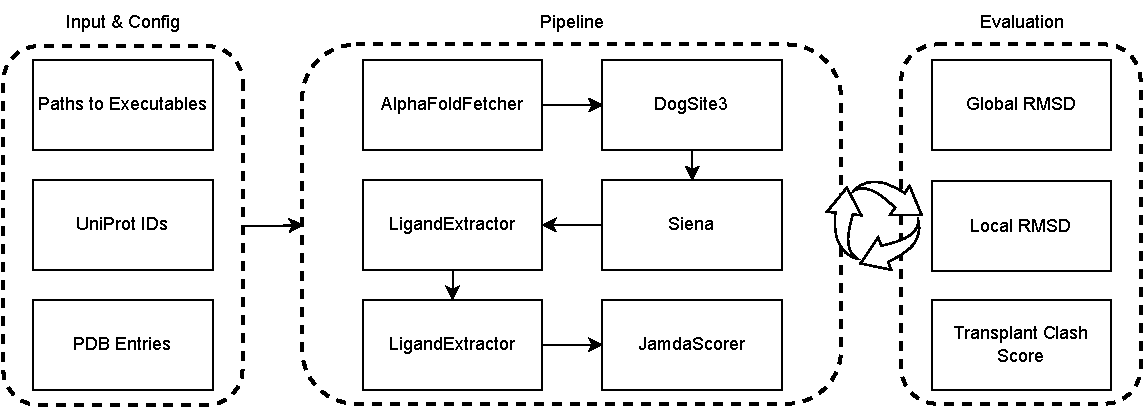
\includegraphics[width=\linewidth]{figures/pipeline_overview.drawio.pdf}
    \caption{High-level pipeline stages: data acquisition; binding site and ligand characterization; alignment and geometric mapping; transplantation; filtering and scoring; evaluation and visualization.}
    \label{fig:pipeline_overview}
\end{figure}


\section{Data and Inputs}
\Todo{Describe the input protein models (AlphaFold/UniProt IDs), how they are fetched, and the benchmark dataset in evaluation/data (size, selection criteria). Include table summarizing proteins used.}
\Todo{Specify configuration via config.toml: key parameters (alignment thresholds, filters), seeds, and runtime knobs.}

\section{Components and Tools}
\subsection{AlphaFold Fetcher}\label{subsec:alphafold_fetcher}

Predicted target structures are sourced from the public AlphaFold Protein Structure Database \cite{jumperHighlyAccurateProtein2021,abramsonAccurateStructurePrediction2024}. For each UniProt accession $U$, the fetcher attempts to download the most recent single-chain model file in Protein Data Bank (PDB) format using the canonical URL pattern:
\begin{center}
    \texttt{https://alphafold.ebi.ac.uk/files/AF-$U$-F1-model\_v4.pdb}
\end{center}
If version \texttt{v4} is not available (HTTP 404), a controlled fallback to \texttt{model\_v3} is performed. This ordered fallback (v4 $\rightarrow$ v3) guarantees maximal currency while preserving compatibility with accessions that have not yet been reprocessed in later database releases. Network and HTTP errors are logged with structured messages; only a definitive failure after exhausting all configured versions raises a terminal exception. The module is deliberately side effect free beyond file system writes and thus supports higher-level retry logic if desired.

All AlphaFold downloads for a run are stored under a deterministic cache directory \texttt{AlphaFold/} inside the tool's designated output root to enable re-use across downstream stages and future executions. File names are preserved verbatim from the source (e.g., \texttt{AF-<UniProt>-F1-model\_v4.pdb}) to maintain traceability to the original database asset. A processed companion file suffixed \texttt{\_processed.pdb} is generated (see below), allowing both raw and normalized forms to coexist. While the current implementation always overwrites existing files (ensuring freshness), the presence of both raw and processed variants provides an implicit cache that higher orchestration layers may exploit to skip redundant network access.

\paragraph{Confidence-Guided Segment Trimming.} AlphaFold supplies per-residue predicted Local Distance Difference Test (pLDDT) scores encoded in the B-factor column of each ATOM record. Rather than discarding individual residues below a threshold (which can produce fragmented backbones and complicate pocket computations), the fetcher applies a conservative \emph{segment-based} pruning strategy: any contiguous stretch of $\ge 5$ residues where \mbox{pLDDT $< 50$} for all members is removed in its entirety. The threshold of 50 aligns with AlphaFold's published qualitative confidence bands (``low'' confidence boundary) and has been widely adopted to demarcate regions likely to be disordered or spuriously modeled; requiring a minimal run length of five suppresses noise from isolated low-scoring residues embedded in otherwise reliable context. This approach preferentially excises flexible termini or unresolved loops while preserving internal residues that might transiently dip below the cutoff.

Implementation-wise, the parser performs two passes over the PDB text: (i) extraction of an ordered residue identifier and associated pLDDT stream (residue identity is defined by concatenated residue name, chain identifier, and sequence number parsed from columns 18--26), and (ii) identification and marking of qualifying low-confidence segments. A second traversal writes out all ATOM/HETATM lines not belonging to flagged segments. Non-coordinate records (HEADER, REMARK, etc.) are retained verbatim to preserve provenance metadata. The output is emitted to \texttt{AF-<UniProt>-F1-model\_vX\_processed.pdb} (same directory) enabling deterministic downstream referencing.

\paragraph{Normalization and Structural Assumptions.} AlphaFold monomer models are emitted as a single chain (commonly chain \texttt{A}); alternative location indicators and insertion codes are not expected and are therefore passed through without modification if present. No coordinate re-numbering or chain renaming is performed, preserving direct comparability with original residue numbering and external annotations (e.g., UniProt feature mappings). Because trimming physically removes ATOM records, residue numbering may exhibit gaps; downstream components treat numbering symbolically and do not require continuity. The fetcher does not currently remap sequence indices nor generate masks; omission is intentional to keep a faithful structural subset rather than a padded representation.

\paragraph{Error Handling and Logging.} Each retrieval attempt logs: (i) target accession and version, (ii) URL, (iii) success or specific failure classification (404 vs. other HTTP vs. network). Processing anomalies (file read/write errors, malformed ATOM records) are trapped and surfaced with contextual messages while falling back to the unprocessed file if trimming cannot be completed safely. This defensive design prevents a single malformed record from aborting an otherwise usable structure.

\paragraph{Limitations and Future Extensions.} The current segment detection logic infers residue boundaries from repeating per-atom records and assumes uniform pLDDT within a residue (fulfilled in AlphaFold outputs). Multi-chain assemblies (e.g., AlphaFold multimer) and partial models are out of scope but could be supported by iterating per chain. Optional future enhancements include: checksum-based cache validation to avoid redundant downloads, configurable pLDDT thresholds and minimal segment length, generation of a residue-level confidence mask, and integration of model confidence metrics (PAE matrices) for region-aware downstream weighting.

Overall, this module provides a reproducible, transparent acquisition and normalization layer that supplies structurally cleaner models to pocket detection and alignment stages while retaining provenance and enabling straightforward parameterization.


\subsection{Binding Site Prediction (DoGSite3)}
Binding pocket detection on the (optionally confidence-trimmed) AlphaFold target model is performed with DoGSite3 \cite{graefBindingSiteDetection2023}, a reimplementation of the original DoGSite approach employing a Difference-of-Gaussians (DoG) filtering scheme on a three-dimensional grid discretization of the solvent-accessible protein envelope. The method locally contrasts a pair of Gaussian-smoothed molecular surface occupancy grids at different scales to accentuate cavity voxels, followed by region growing, connectivity refinement, and physicochemical descriptor calculation. Compared to its predecessor, DoGSite3 emphasizes robustness in the presence of bound ligands and yields reproducible pocket rankings with reduced parameter sensitivity (see publication for benchmarked performance characteristics). We treat its ranked pocket list as a proxy for ligandable micro-environments in subsequent donor alignment.

\paragraph{Invocation and Output Layout.} Execution is wrapped by the Dogsite3 tool adapter (see implementation in \texttt{foldfusion/tools/dogsite3.py}), which constructs a deterministic command line:
\begin{center}
    \texttt{<dogsite3> --proteinFile <ABSOLUTE\_PDB\_PATH> --writeSiteResiduesEDF}
\end{center}
where \texttt{<dogsite3>} denotes the configured executable path and the input PDB path is resolved to an absolute canonical location prior to invocation. All artifacts are written into a run-scoped directory \texttt{Dogsite3/} underneath the tool's designated output root (one directory per target). The \texttt{--writeSiteResiduesEDF} flag instructs DoGSite3 to emit per-pocket EDF (``Extended Descriptor File'') records that include residue membership annotations in addition to geometric and physicochemical attributes.

\paragraph{Pocket Selection and EDF Normalization.} For each target we currently retain only the top-ranked pocket as defined by DoGSite3's internal scoring (exposed as index 1 in the output file name pattern). The corresponding EDF is expected at \texttt{Dogsite3/output\_P\_1\_res.edf}.

Immediately post-run the adapter performs an idempotent sanitization step: if the EDF header line \texttt{REFERENCE <NO-FILE>} is present, it is replaced in-place with the absolute path to the analyzed PDB file. This guarantees downstream tools (notably the SIENA binding-site similarity search) have a resolvable pointer without relying on relative directory context. No other EDF fields are modified, and the operation is skipped if a valid \texttt{REFERENCE} already exists.

\paragraph{Extracted Features Consumed Downstream.} The EDF encapsulates a mixture of scalar descriptors and residue-level membership annotations. While DoGSite3 enumerates an extended descriptor set, the current pipeline utilizes the following subset in later decision functions and reporting:
\begin{itemize}
    \item Geometric: pocket volume, surface area, effective radius / diameter, and asphericity---used to characterize cavity size and shape when comparing donor pockets or rationalizing ligand accommodation.
    \item Physicochemical composition: hydrophobic surface fraction, polar surface fraction, hydrogen bond donor/acceptor counts, aromatic residue count—informing plausibility of transplanted ligand physicochemical complementarity.
    \item Accessibility: mouth opening area and enclosure metrics—qualitatively referenced when interpreting steric clash filtering outcomes.
    \item Ranking / score: the native DoGSite3 pocket score employed only implicitly (selection of rank 1 pocket) but retained for audit.
    \item Residue membership list: chain identifiers and residue numbers forming the pocket environment; projected onto alignment results to compute overlap and to guide ligand clash resolution.
\end{itemize}
Additional descriptors present in the EDF (e.g., curvature-derived terms) are stored but not presently incorporated into filtering heuristics; preservation ensures future extension does not require regeneration of pockets. All EDF files are version-stamped implicitly through inclusion of the upstream executable version (recorded in the structured log) facilitating reproducibility and cross-run comparison.

In preliminary internal tests (evaluating downstream SIENA hit quality, ligand transplantation success, and final filtering yield) inclusion of additional pockets beyond rank 1 (evaluated up to the top 5) produced no measurable improvement while increasing wall-clock time. Consequently, to avoid unnecessary runtime expansion and complexity, the pipeline currently restricts processing to the single top-ranked pocket.

Overall, this stage converts a raw target structure into a normalized pocket descriptor and residue environment bundle with explicit provenance, enabling reproducible, tool-version aware propagation of binding-site context into alignment and ligand transfer stages.

\subsection{Donor Databases and Retrieval (PDB/UniProt/SIENA DB)}
Donor structures (experimental templates and their cognate ligands) are sourced from a locally mirrored slice of the Protein Data Bank (PDB) \cite{burleyRCSBProteinData2019}. Mirroring is performed via \texttt{rsync} using the template script distributed by RCSB (adapted in \texttt{scripts/rsyncPBD.sh}); only the classic PDB coordinate hierarchy \texttt{data/structures/divided/pdb/} is synchronized to reduce footprint. We employ the RCSB public rsync endpoint (port 33444) and capture the mirror date/time stamp in the run metadata. The mirror path (default \texttt{/home/marius/Data/pdb}) is treated as read-only by the pipeline. Periodic refresh (manually triggered) ensures currency while preserving deterministic snapshots between updates. Each run logs the PDB snapshot date plus the total number of mirrored entries, enabling exact reconstruction of the donor corpus.

UniProt accessions serve as the primary identifiers for targets (AlphaFold models) and provide linkage to experimental structures through canonical mapping tables (implicit in AlphaFold naming conventions). While a separate UniProt flat file is not parsed here, consistency of residue numbering and chain semantics is preserved by deferring any sequence-based reconciliation to later alignment stages; provenance of donor sequences thus remains anchored to their deposited PDB records.

To accelerate binding-site similarity searches, a SIENA structure database is built (or re-used if present) using the SienaDB tool wrapper (implementation: \texttt{foldfusion/tools/siena\_db.py}), referencing the method described in \cite{bietzSIENAEfficientCompilation2016}. Database creation indexes residue-kmer encodings across all mirrored PDB entries, enabling sub-second retrieval of alternative binding site conformations that share local sequence/structural motifs with the query pocket. The generator is invoked once per run with arguments:
\begin{center}
    \texttt{<siena\_db\_build> --database <NAME> --directory <MIRROR\_PDB\_DIR> --format <f>}
\end{center}
where \texttt{<f>} is \texttt{1} for plain \texttt{.pdb} files (current configuration) or \texttt{0} if operating on compressed legacy \texttt{.ent.gz} layouts. The wrapper accepts an optional explicit path; otherwise it defaults to \texttt{<output>/SienaDB/siena\_db}. Post-build, the code accommodates ambiguity in produced filenames (with or without a \texttt{.db} suffix) by detecting and adopting the existing variant to avoid downstream path mismatches.

\paragraph{Regeneration and Validity Checks.} Prior to invocation, the wrapper performs existence and plausibility validation: (i) file presence, (ii) regular file type, and (iii) a minimal size threshold ($ < 1 KB$ flagged as invalid). If these criteria are satisfied, regeneration is skipped and the existing index reused, ensuring stable identifiers and minimizing unnecessary I/O. Otherwise, a fresh index is created in-place. This behavior enforces idempotence: repeated runs over an unchanged PDB mirror are constant-time with respect to database preparation.

\paragraph{Directory Layout and Provenance.} All generated index artifacts reside under \texttt{SienaDB/} inside the run's output root (or a user-specified directory if an absolute database path is given). Structured logs record: executable path and (if available) version string, build timestamp, input directory hash (optional future extension), database file size, and number of processed PDB entries. These annotations collectively permit reproducibility assessments and forensic reconstruction of search scope.

\paragraph{Donor Structure Filtering.} A light-weight, pre-alignment filtering regime is applied conceptually (some criteria enforced implicitly by tool behaviour, others by configuration) to exclude low-informative or incompatible donors:
\begin{itemize}
    \item \textbf{Experimental resolution:} Structures exceeding a configured maximal resolution (e.g., \(\ge 3.0 \AA\); crystallography only) are candidates for exclusion to reduce noise from poorly resolved active sites.
    \item \textbf{Polymer type:} Only protein chains (standard amino acid polymers) are considered; nucleic acid or hybrid complexes contribute coordinates but are not indexed as donors for binding site transplantation.
    \item \textbf{Ligand presence:} Preference is given to entries containing at least one non-solvent, non-polymer ligand within the pocket vicinity (enabling later ligand transfer); purely apo conformations remain permissible when needed for conformational diversity.
    \item \textbf{Model completeness:} Grossly truncated chains or entries dominated by unresolved (missing) residues can be pruned (future automated metric—currently manual oversight via log summaries).
    \item \textbf{Redundancy control:} Intrinsic redundancy is implicitly mitigated by SIENA's k-mer indexing; optional explicit sequence identity clustering (not yet enabled) is noted as a scalable extension.
\end{itemize}
At this stage, filtering is conservative to preserve conformational breadth; more stringent quality and conflict assessments occur after pocket-level alignment and ligand transplantation.

\paragraph{Ligand Data.} Ligands are leveraged directly from donor PDB HETATM records; no external ligand database normalization is imposed in this stage. Retained hetero groups exclude water and common crystallization additives (handled via a configurable exclusion list, future explicit parameterization). Ligand identifiers and residue numbering propagate unchanged, enabling traceable mapping during transplantation and optimization (JAMDA stage).

\paragraph{Versioning and Snapshot Notation.} Each results set (alignments, transplanted ligands, scores) references: (i) PDB snapshot date, (ii) SIENA database file checksum (future extension), and (iii) AlphaFold model version for the target. This triad forms the minimal provenance key required to reproduce donor retrieval decisions. Inclusion of exact rsync command options (logged verbatim from \texttt{rsyncPBD.sh}) further aids auditability.

In summary, this component assembles a high-quality yet breadth-preserving donor search space through a reproducible mirror, a lazily materialized SIENA index, and light-touch structural filtering, establishing the foundation for subsequent pocket similarity search and targeted ligand transplantation.

\subsection{Binding-Site Similarity Search and Alignment (SIENA)}
\Todo{Describe inputs (EDF pocket from DoGSite3) and the SIENA search/alignment workflow; include citation and tool version.}
\Todo{Document command parameters used: \texttt{--edf}, \texttt{--database}, \texttt{--output .}, identity cutoff (\texttt{--identity 0.85}); justify chosen thresholds.}
\Todo{Explain result parsing: reading \texttt{resultStatistic.csv} (semicolon separated), column cleanup, sorting primarily by Active site identity (desc), then Backbone and All-atom RMSD (asc).}
\Todo{Clarify use of \texttt{ensemble/\*.pdb} files for downstream ligand extraction/transplantation and how many top alignments are retained (configurable \texttt{siena\_max\_alignments}).}

\subsection{Ligand Optimization and Scoring (JAMDA)}
\Todo{Summarize JAMDA's role: energy-based pose optimization/scoring of transplanted ligands; include citation and tool version.}
\Todo{Describe invocation pattern per ligand: inputs (AlphaFold PDB, ligand SDF), outputs (optimized SDF), and flags used (\texttt{--optimize}); output organization (\texttt{JamdaScorer/<PDB>/ligand\_id.sdf}).}
\Todo{State what scores/outputs are captured and how they inform filtering (e.g., clash reduction, score improvements). Cross-reference concrete thresholds in Filtering and Scoring.}
\subsection{Alignment}
\Todo{Describe global/local alignment methods used; define RMSD/score variants and parameters.}
\subsection{Transplantation}
\Todo{Explain coordinate mapping, handling of alternate locations, protonation states, and chain/residue mapping.}
\subsection{Filtering and Scoring}
\Todo{Define clash checks, distance cutoffs, and quality indicators; justify chosen thresholds. Reference how SIENA metrics (identity, RMSDs) and JAMDA outputs contribute to accept/reject decisions.}

\section{Implementation Details}
\Todo{Summarize code structure (packages in foldfusion/), logging, CLI entry points, and dependency management (pyproject/uv.lock).}
\Todo{Discuss error handling and retries for external resources; note offline/cached mode.}

\section{Reproducibility}
\Todo{Document exact environment (Python version, key packages), compute hardware, and commands to reproduce results. Reference Appendix for full config and commit hash.}

\section{Ethical and Licensing Considerations}
\Todo{Note database/tool licenses and usage restrictions; acknowledge limitations of homology-based inference.}
